% mnras_template.tex
%
% LaTeX template for creating an MNRAS paper
%
% v3.0 released 14 May 2015
% (version numbers match those of mnras.cls)
%
% Copyright (C) Royal Astronomical Society 2015
% Authors:
% Keith T. Smith (Royal Astronomical Society)

% Change log
%
% v3.0 May 2015
%    Renamed to match the new package name
%    Version number matches mnras.cls
%    A few minor tweaks to wording
% v1.0 September 2013
%    Beta testing only - never publicly released
%    First version: a simple (ish) template for creating an MNRAS paper

%%%%%%%%%%%%%%%%%%%%%%%%%%%%%%%%%%%%%%%%%%%%%%%%%%
% Basic setup. Most papers should leave these options alone.
\documentclass[fleqn,usenatbib,useAMS]{mnras}

% MNRAS is set in Times font. If you don't have this installed (most LaTeX
% installations will be fine) or prefer the old Computer Modern fonts, comment
% out the following line
%\usepackage{newtxtext,newtxmath}violet
% Depending on your LaTeX fonts installation, you might get better results with one of these:
\usepackage{mathptmx}
%\usepackage{txfonts}

% Use vector fonts, so it zooms properly in on-screen viewing software
% Don't change these lines unless you know what you are doing
\usepackage[T1]{fontenc}
\usepackage{ae,aecompl}


%%%%% AUTHORS - PLACE YOUR OWN PACKAGES HERE %%%%%

% Only include extra packages if you really need them. Common packages are:
\usepackage{graphicx}	% Including figure files
\usepackage{amsmath}	% Advanced maths commands
\usepackage{amssymb}	% Extra maths symbols
\usepackage{bm}		% Bold maths symbols, including upright Greek
\usepackage{pdflscape}	% Landscape pages
\usepackage{color}
\usepackage{exscale}
\usepackage{natbib}
\usepackage{rotating}
\usepackage{rotate}
\usepackage{afterpage}
\usepackage{booktabs,threeparttable}
\usepackage{relsize}
\usepackage{lscape}
\usepackage{tabularx}
\usepackage{longtable}
\usepackage{ltxtable}
\usepackage{txfonts}
\usepackage{bbm}
\usepackage{widetext}
\usepackage{subfig}

% Bibliography and bibfile
% Taken from aa.cls
\def\aj{AJ}%
          % Astronomical Journal
\def\araa{ARA\&A}%
          % Annual Review of Astron and Astrophys
\def\apj{ApJ}%
          % Astrophysical Journal
\def\apjl{ApJ}%
          % Astrophysical Journal, Letters
\def\apjs{ApJS}%
          % Astrophysical Journal, Supplement
\def\ao{Appl.~Opt.}%
          % Applied Optics
\def\apss{Ap\&SS}%
          % Astrophysics and Space Science
\def\aap{A\&A}%
          % Astronomy and Astrophysics
\def\aapr{A\&A~Rev.}%
          % Astronomy and Astrophysics Reviews
\def\aaps{A\&AS}%
          % Astronomy and Astrophysics, Supplement
\def\azh{AZh}%
          % Astronomicheskii Zhurnal
\def\baas{BAAS}%
          % Bulletin of the AAS
\def\jrasc{JRASC}%
          % Journal of the RAS of Canada
\def\memras{MmRAS}%
          % Memoirs of the RAS
\def\mnras{MNRAS}%
          % Monthly Notices of the RAS
\def\pra{Phys.~Rev.~A}%
          % Physical Review A: General Physics
\def\prb{Phys.~Rev.~B}%
          % Physical Review B: Solid State
\def\prc{Phys.~Rev.~C}%
          % Physical Review C
\def\prd{Phys.~Rev.~D}%
          % Physical Review D
\def\pre{Phys.~Rev.~E}%
          % Physical Review E
\def\prl{Phys.~Rev.~Lett.}%
          % Physical Review Letters
\def\pasp{PASP}%
          % Publications of the ASP
\def\pasj{PASJ}%
          % Publications of the ASJ
\def\qjras{QJRAS}%
          % Quarterly Journal of the RAS
\def\skytel{S\&T}%
          % Sky and Telescope
\def\solphys{Sol.~Phys.}%
          % Solar Physics
\def\sovast{Soviet~Ast.}%
          % Soviet Astronomy
\def\ssr{Space~Sci.~Rev.}%
          % Space Science Reviews
\def\zap{ZAp}%
          % Zeitschrift fuer Astrophysik
\def\nat{Nature}%
          % Nature
\def\iaucirc{IAU~Circ.}%
          % IAU Cirulars
\def\aplett{Astrophys.~Lett.}%
          % Astrophysics Letters
\def\apspr{Astrophys.~Space~Phys.~Res.}%
          % Astrophysics Space Physics Research
\def\bain{Bull.~Astron.~Inst.~Netherlands}%
          % Bulletin Astronomical Institute of the Netherlands
\def\fcp{Fund.~Cosmic~Phys.}%
          % Fundamental Cosmic Physics
\def\gca{Geochim.~Cosmochim.~Acta}%
          % Geochimica Cosmochimica Acta
\def\grl{Geophys.~Res.~Lett.}%
          % Geophysics Research Letters
\def\jcap{JCAP}%
          % Journal of Cosmology and Astroparticle Physics
\def\jcp{J.~Chem.~Phys.}%
          % Journal of Chemical Physics
\def\jgr{J.~Geophys.~Res.}%
          % Journal of Geophysics Research
\def\jqsrt{J.~Quant.~Spec.~Radiat.~Transf.}%
          % Journal of Quantitiative Spectroscopy and Radiative Trasfer
\def\memsai{Mem.~Soc.~Astron.~Italiana}%
          % Mem. Societa Astronomica Italiana
\def\nphysa{Nucl.~Phys.~A}%
          % Nuclear Physics A
\def\physrep{Phys.~Rep.}%
          % Physics Reports
\def\physscr{Phys.~Scr}%
          % Physica Scripta
\def\planss{Planet.~Space~Sci.}%
          % Planetary Space Science
\def\procspie{Proc.~SPIE}%
          % Proceedings of the SPIE



%%%%%%%%%%%%%%%%%%%%%%%%%%%%%%%%%%%%%%%%%%%%%%%%%%
%%%%% AUTHORS - PLACE YOUR OWN COMMANDS HERE %%%%%
\newcommand{\tbf}{\textbf}
\newcommand{\ti}{\textit}

\newcommand{\bea}{\begin{eqnarray}}
\newcommand{\be}{\begin{equation}}
\newcommand{\ben}{\begin{enumerate}}
\newcommand{\bi}{\begin{itemize}}
\newcommand{\eea}{\end{eqnarray}}
\newcommand{\ee}{\end{equation}}
\newcommand{\ei}{\end{itemize}}
\newcommand{\een}{\end{enumerate}}
\newcommand{\nn}{\nonumber}
\newcommand{\vpi}{\mathbf \pi}
\newcommand{\vecd}{\mathbf d}
\newcommand{\matC}{\mathbf C}
\newcommand{\matQ}{\mathbf Q}
\newcommand{\ensav}[1]{\left\langle #1 \right\rangle}
\def\bfp{\mbox{\bf p}}
\def\bfq{\mbox{\bf q}}
\def\bfk{\mbox{\bf k}}
\def\bfr{\mbox{\bf r}}

\newcommand{\like}{L}
\newcommand{\prob}{P}
\newcommand{\probr}{P_r}
\newcommand{\p}{\vek p}
\newcommand{\pco}{\vek p_\mr{c}}
\newcommand{\pnu}{\vek p_\mr{n}}
\newcommand{\plf}{\vek p_\mr{LF}}
\newcommand{\D}{\vek D}
\newcommand{\Del}{\vek \Delta}
\newcommand{\M}{\vek M}
\newcommand{\N}{\vek N}
\newcommand{\U}{\vek U}


\newcommand{\om}{\Omega_\mr m}
\newcommand{\omb}{\Omega_\mr b}
\newcommand{\sig}{\sigma_8}
\newcommand{\ns}{n_s}
\newcommand{\w}{w_0}
\newcommand{\wa}{w_a}

\renewcommand{\d}{{\rm d}}
\newcommand{\pd}{P_{\delta}}
\newcommand{\pe}{P_\mr E}

\newcommand{\vt}{\vartheta}
\newcommand{\vp}{\varphi}
\newcommand{\eps}{\epsilon}
\newcommand{\abs}[1]{| #1 |}
\newcommand{\mr}{\mathrm}

\newcommand{\vek}{\mathbf}
\newcommand{\bs}{\boldsymbol}

\newcommand{\tim}[1]{\textcolor{blue}{\textbf{[Tim: #1]}}}
\newcommand{\eli}[1]{\textcolor{green}{\textbf{[Eli: #1]}}}
\newcommand{\todo}[1]{\textcolor{red}{\textbf{[todo: #1]}}}

\voffset=-0.5in

\newcommand{\red}[1]{\textcolor{red}{#1}}

%%%%%%%%%%%%%%%%%%%%%%%%%%%%%%%%%%%%%%%%%%%%%%%%%%

%%%%%%%%%%%%%%%%%%% TITLE PAGE %%%%%%%%%%%%%%%%%%%

\title[Cosmology from WFIRST - Synergies with LSST]{Cosmology from WFIRST - Synergies with LSST}

\author[Tim Eifler]{Tim Eifler$^{1}$\thanks{E-mail: timeifler@email.arizona.edu}, Melanie Simet$^{2}$, Elisabeth Krause$^{1}$, Chris Hirata$^{3}$, Chen Heinrich$^{4}$\\
% List of institutions
$^{1}$ Department of Astronomy/Steward Observatory, University of Arizona, 933 North Cherry Avenue, Tucson, AZ 85721-0065, USA \\
$^{2}$ Department of Physics and Astronomy, University of California Riverside, 900 University Ave, Riverside, CA 92521, USA \\
}


\begin{document}

\date{Accepted . Received ; in original form }

\pagerange{\pageref{firstpage}--\pageref{lastpage}} \pubyear{2014}

\maketitle

\label{firstpage}

\begin{abstract}
We explore synergies between the ground-based Large Synoptic Survey Telescope (LSST) and the space-based Wide-Field Infrared Survey Telescope (WFIRST). In particular, we consider a scenario where the currently envisioned survey strategy for WFIRST's High Latitude Survey (HLS), i.e. 2000 deg$^2$ in four narrow photometric bands is changed in favor of a strategy that combines rapid coverage of the LSST area in just one broad band followed by a smaller area covered in the four narrow bands. 

We find ....
%We compare the cosmological constraining power for a joint weak lensing and galaxy clustering analysis (so-called 3x2pt) LSST and WFIRST individually and in combination given the new strategy. 
%
%from the individual survey endeavors as currently planned and By the time WFIRST launches, LSST will have been in survey mode for several years already and will have built up substantial survey depth and area. The science collaborations of LSST will know what limits the precision of their core science cases and what type of space observations are most valuable to overcome key systematic uncertainties. WFIRST, with its broad range of capabilities, will be an ideal partner observatory to LSST at exactly the right time.
%
%In this paper we outline two concepts for joint survey scenarios: The first is a 5-month, wide WFIRST survey in one band that would cover the full LSST survey area. This 5-month endeavor would provide high-resolution imaging for $>$95\% of the LSST Year 10 weak lensing galaxy sample. The second scenario is a 1.5-year wide WFIRST survey in one band that would cover the full LSST survey area. For this second scenario we explore the joint LSST+WFIRST science return on cosmic acceleration from a joint weak lensing and galaxy clustering analysis. 
%
%The combination of space-based resolution, color information from the ground, and infrared coverage from space over 18,000 deg$^2$ would enable a new level of precision for the existing core science cases of both experiments. It is now timely for WFIRST and LSST to set up a joint survey optimization and systematics mitigation effort that maximizes the science return for the community from the next decade's flagship experiments in survey cosmology.

\end{abstract}


\begin{keywords}
cosmological parameters -- theory --large-scale structure of the Universe
\end{keywords}

\renewcommand{\thefootnote}{\arabic{footnote}}
\setcounter{footnote}{0}


\section{Introduction}
\label{sec:intro}
Observing the formation and evolution of the large-scale structure in our Universe provides a wealth of cosmological information and allows us to constrain fundamental physics questions such as the nature of dark energy, the mass and number of species of neutrinos, possible modifications to general relativity as a function of scale or environment, or the nature of dark matter interactions. 

Early results from the Dark Energy Survey (DES\footnote{www.darkenergysurvey.org/}), the Kilo-Degree Survey (KiDS\footnote{http://www.astro-wise.org/projects/KIDS/}), and the Hyper Suprime Cam (HSC\footnote{http://www.naoj.org/Projects/HSC/HSCProject.html}) have demonstrated the feasibility of complex analyses from photometric data. 

The next decade will provide cosmologists with a wealth of survey data from various, highly complementary experiments. 

The Wide Field Infrared Survey Telescope (WFIRST), scheduled to start mid 2020s, is a versatile space-based observatory, covering science cases from exoplanets to galaxy evolution to fundamental physics \citep{2019arXiv190205569A}. WFIRST's High Latitude Survey (HLS)\footnote{WFIRST} is designed to constrain dark energy evolution and deviations from GR with exquisite control of systematics. The WFIRST HLS survey ensures excellent systematics control via space-quality imaging, photometry across 4 NIR bands, a 0.28 deg$^2$ field of view with a 0.11 arcsec pixel scale, and a $\sim$600 resolution grism enabling deep spectroscopic galaxy redshift measurements over the same survey area as the imaging survey. The envisioned survey area of 2000 deg$^2$ is covered by WFIRST in 1.6 years both in the imaging and spectroscopic component. 


The Large Synoptic Survey Telescope (LSST) \citep{2009arXiv0912.0201L}, scheduled to be fully operational in the early 2020s, will provide the cosmology community with an unprecedented amount of high quality data from the ground. LSST will cover 18,000 deg$^2$ every 3 nights in 6 visible bands and flood the community with $\sim$20TB of imaging data per day, which will be highly synergistic to several other science endeavors in the 2020s. LSST is of course limited by the atmosphere in terms of seeing and wavelength coverage. For dark energy and other science cases the issue of blended galaxies \citep{2016ApJ...816...11D} is a potential limiting systematic uncertainty for galaxy shape and photo-z measurements.  

In this paper we focus on synergies between WFIRST and LSST, specifically we explore alterations to the WFIRST observing strategy that maximize said synergies. Rather than considering WFIRST's HLS  in its current form, we consider instead the versatile capabilities of the WFIRST observatory (cf.~Fig.~\ref{fi:wfirstabilities}), and outline alternative scenarios that make the best use of WFIRST capabilities in partnership with LSST.


\section{The WFIRST mission \todo{Need someone to read and verify/smooth}}

 \begin{figure}
  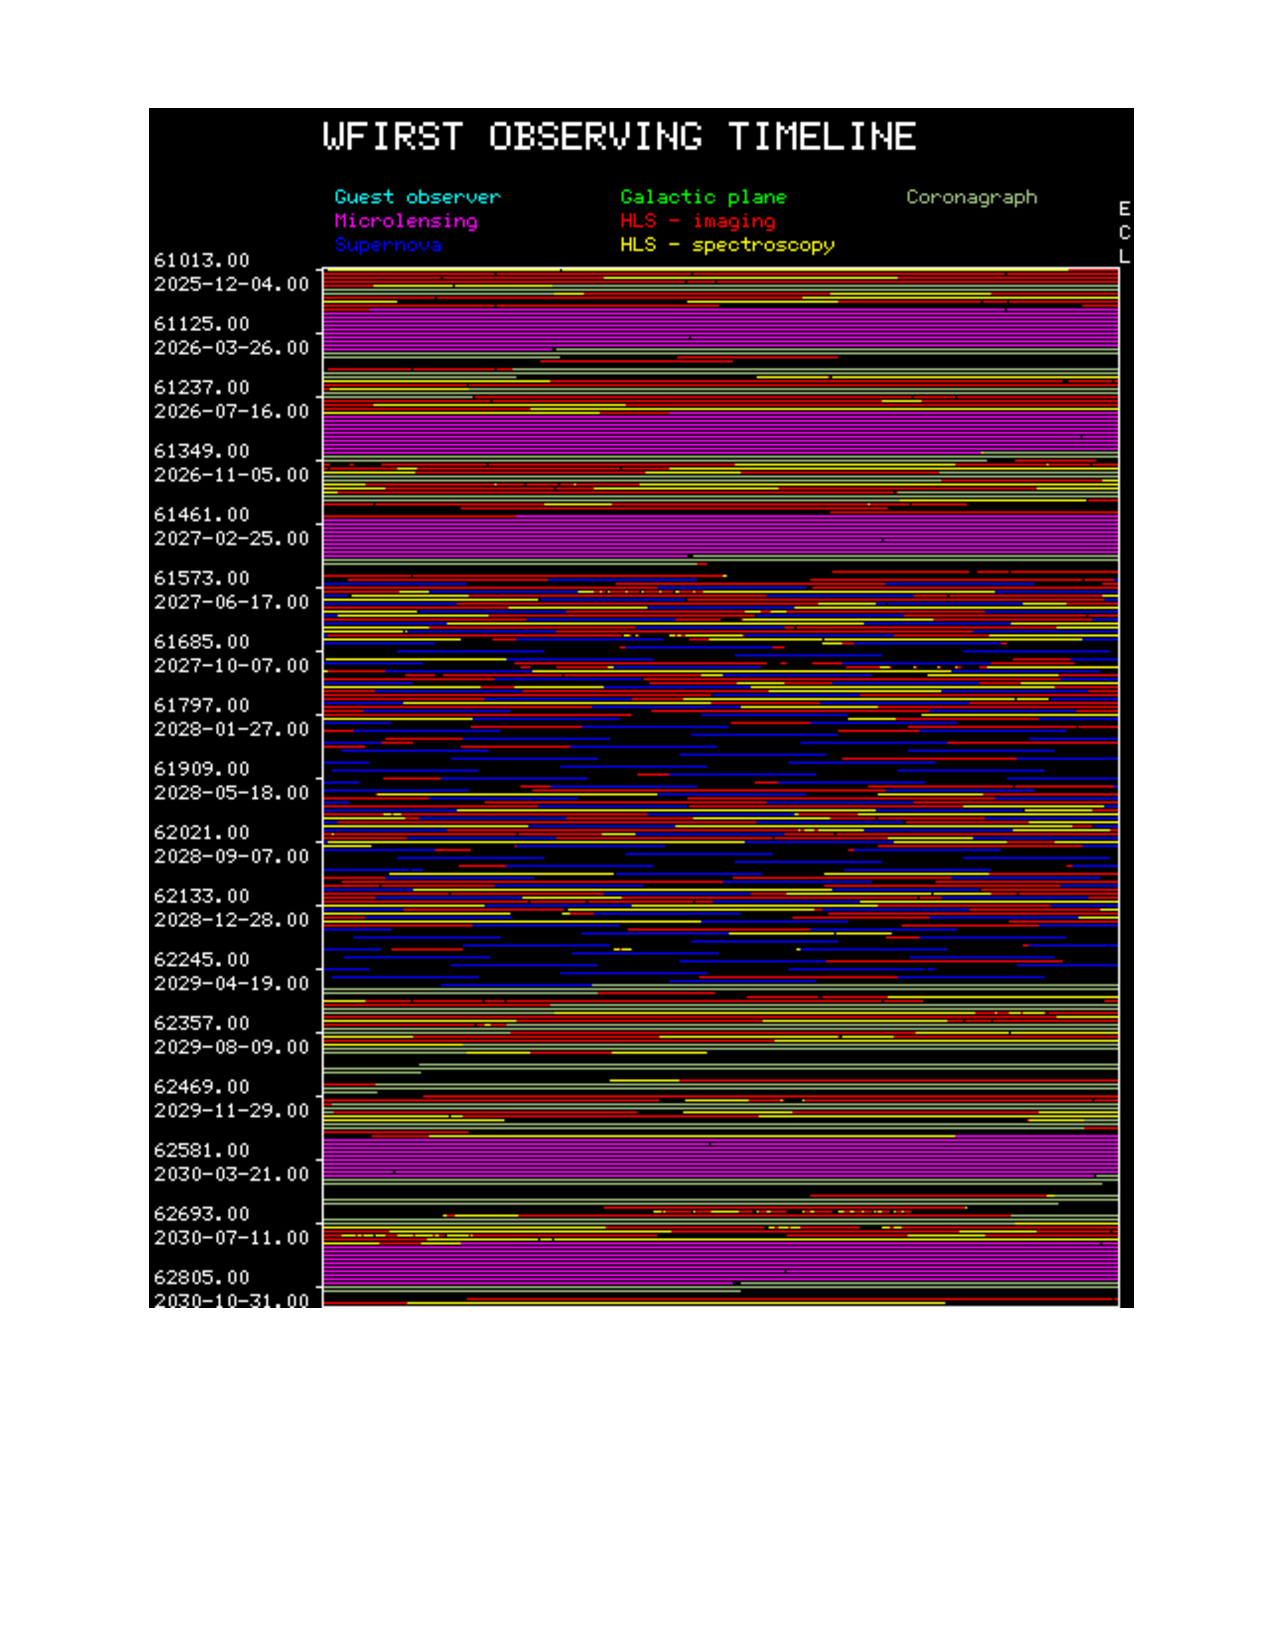
\includegraphics[width=8.5cm]{plots/WFIRST_timeline.pdf}
\caption{An example WFIRST survey strategy as taken from the SDT 2015 report \citep{spergel15} and computed from the ETC v0.13 \citep{hirata13??}. The individual survey components are colored into the timeline graphic: blue for the SN survey, Magenta for Microlensing, Red and Yellow for the HLIS and HLSS, respectively. The remaining time will be allocated as guest observer proposals to the science community.}
\label{fi:timeline}
\end{figure}





WFIRST is  planned to launch in the mid 2020's into  the L2 orbit with a nominal mission length of 6 years. Its primary mirror measures 2.37 m and is equipped with a wide field instrument containing the wide field channel (WFC) primarily used by the High Latitude Survey. The WFC is composed of a 3x6 array,  each containing 4k x 4k HgCdTe IR detectors, yielding an effective FoV of 0.281 deg$^2$. This FoV is about a factor of $\sim$200 larger than the instruments on HST (WFC3/IR) and JWST (NIRCam), enabling deep sky surveys of unprecedented size. Six imaging filters are used covering the $0.76-2.0$ $\mu$m range. The central wavelengths of filters are 0.87, 1.09, 1.30, 1.60, 1.88, 1.40 $\mu$m and spatial resolution per pixel is 0.11 arcsec. In addition, a grism is used to perform slitless spectroscopy covering the $1.35-1.89$ $\mu$m range (at thermal background of 282K). The grism has a dispersion of $1.04-1.14$ nm per pixel and a spectral resolution $\lambda/\Delta \lambda \approx 622 - 871$ for 2 pixels~\citep{2015arXiv150303757S}. % double check numbers and put in refs.

WFIRST has a 6 year prime mission composed of a 2 year HLS, 6 months of SN observations over 2 years, 1 year each for the exoplanet and microlensing observations, plus a competed Guest Observer program for $>$1.25 years. While the nominal mission is 6 years, there are no consumables to prevent WFIRST from operating for 10 years or more. This is why we also consider extended mission scenarios in this paper for the HLS. Among two-year nominal HLS, 1.3 years is used for imaging and 0.6 years for grism spectroscopy, covering a total of 2000 deg$^2$~\citep{2015arXiv150303757S}. % insert any more comments here (could vary depth etc)



\renewcommand{\arraystretch}{1.3}
\begin{table*}
\caption{Imaging capabilities of WFIRST  and LSST}
\begin{center}
\begin{tabular*}{0.9\textwidth}{@{\extracolsep{\fill}}| c | c c c c c c c |}
\hline
\hline
\multicolumn{8}{|c|}{\tbf{WFIRST Imaging Capabilities \footnote{$https://wfirst.gsfc.nasa.gov/science/WFIRSTScienceSheetFINAL.pdf$}}} \\
\hline 
\multicolumn{2}{|c }{\tbf{Telescope Aperture}}  & \multicolumn{2}{|c }{\tbf{Field of View}} & \multicolumn{2}{|c }{\tbf{Pixel Scale}} & \multicolumn{2}{|c|}{\tbf{Wavelength Range}} \\
\multicolumn{2}{|c }{\tbf{2.4 meter}}  & \multicolumn{2}{|c }{\tbf{0.28 sq deg}} & \multicolumn{2}{|c }{\tbf{0.11 arcsec}} & \multicolumn{2}{|c|}{\tbf{0.5-2.0 $\mu$m}} \\
\hline 
\hline 
Filters & R062 & Z087& Y106 & J129 & H158 & F184 & W146 \\
Wavelength ($\mu$m) & 0.48 - 0.76 & 0.76 - 0.98 & 0.93 - 1.19 & 1.13 - 1.45 & 1.38 - 1.77 & 1.68 - 2.00 & 0.93 -2.00 \\
Sensitivity (5 $\sigma$ AB mag in 1h) &28.5 & 28.02 & 27.95 & 27.87 & 27.81 & 27.32 & 28.33 \\
\hline 
\hline
\end{tabular*}

\vspace{0.4cm}

\begin{tabular*}{0.9\textwidth}{@{\extracolsep{\fill}}| c | c c c c c c |}
\hline
\hline
\multicolumn{7}{|c|}{\tbf{LSST Imaging Capabilities \footnote{$https://www.lsst.org/scientists/keynumbers$}}} \\
\hline 
\multicolumn{2}{|c }{\tbf{Telescope Aperture}}  & \multicolumn{2}{|c }{\tbf{Field of View}} & \multicolumn{2}{|c|}{\tbf{Pixel Scale}} & \tbf{Wavelength Range} \\
\multicolumn{2}{|c }{\tbf{6.67 meter (effective)}}  & \multicolumn{2}{|c }{\tbf{9.62 sq deg}} & \multicolumn{2}{|c| }{\tbf{0.2 arcsec}} & \tbf{0.35 - 1.06 $\mu$m} \\
\hline 
\hline 
Filters & u & g & r & i & z & Y \\
Wavelength ($\mu$m) & 0.324 - 0.395 & 0.405 - 0.552 & 0.552 - 0.691 & 0.691 - 0.818 & 0.818 - 0.921 & 0.922 - 0.997 \\
Sensitivity (5 $\sigma$ AB mag in 1h) &&&&&&\\
\hline 
\hline
\end{tabular*}
\end{center}
\label{tab:params}
\end{table*}
\renewcommand{\arraystretch}{1.0}






\section{Simulating WFIRST observations}
We use the WFIRST exposure time calculator (ETC) in weak lensing mode \citep{2012arXiv1204.5151H} to compute the results of Figs.~\ref{fi:wbanddepth} and \ref{fi:contour_stats}. We fix the time per exposure and vary the number of exposures covering the sky area; total survey time for a given number of exposures includes a simple prescription for overheads and is correct to approximately 10$\%$. 

We closely follow \cite{hcm18} in applying the ETC results to the CANDELS data set \citep{Candels}. The ETC has a built-in option to obtain a weak lensing catalogue based on an input catalogue. We apply this feature to generate the WFIRST lensing sample from the CANDELS catalogue and look up the distribution of magnitudes in the LSST bands for the detected WFIRST galaxies. For LSST, our catalog cuts are based on the galaxy magnitudes and uncertainties in the LSST $i$-band, in particular we assume an LSST weak lensing galaxy sample that includes all galaxies with a $20\sigma$ point detection. After applying these cuts to the CANDELS galaxies we determine the $H$- and $W$-band magnitude distributions. 

For the WFIRST clustering sample we select CANDELS galaxies with S/N$>$10 and again look at the LSST columns to determine whether a detected galaxy in WFIRST is detected at sufficient S/N in the LSST bands to enable ground-based photo-z. 

 \begin{figure*}
  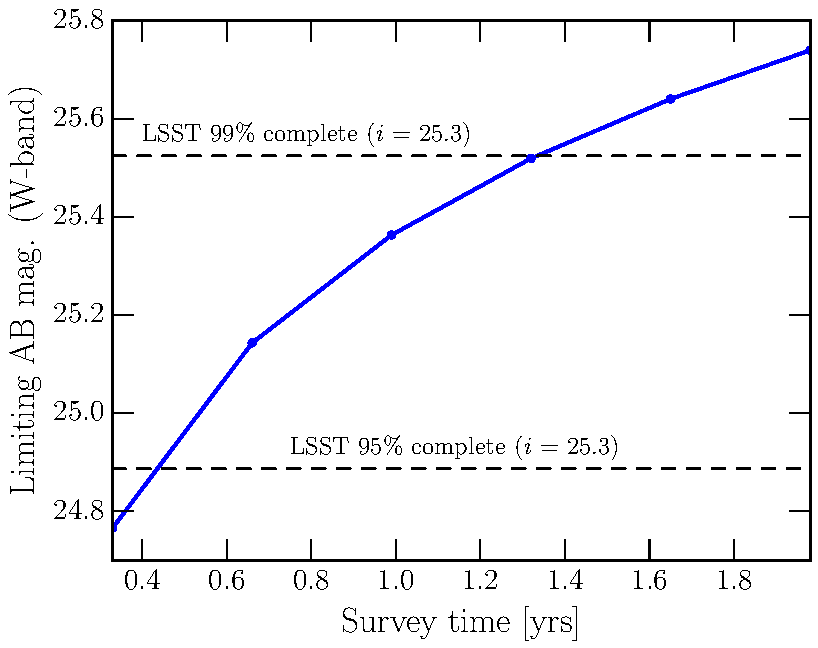
\includegraphics[width=8.3cm]{plots/plot_magnitude_wband.pdf}
  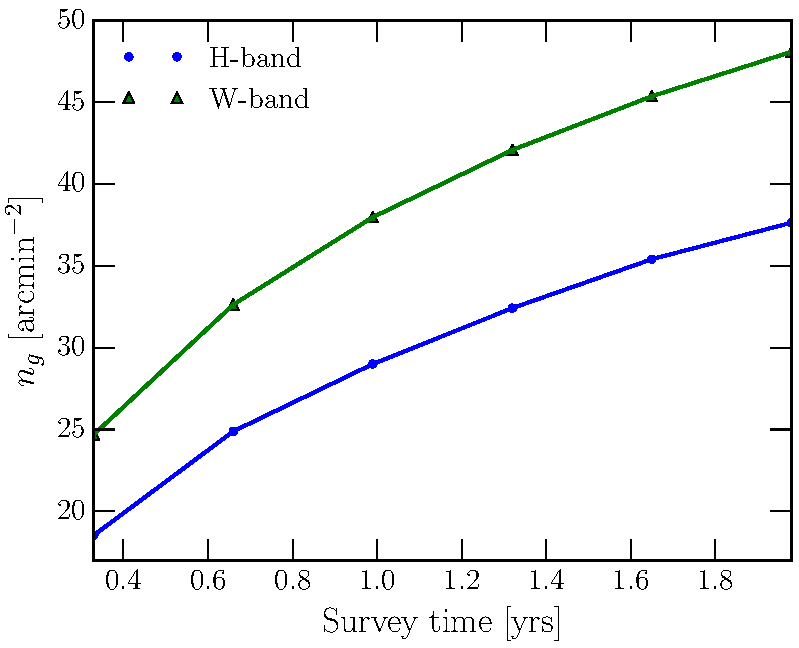
\includegraphics[width=8.1cm]{plots/plot_number_density_hband_and_wband.pdf}
\caption{\textit{Left:} Limiting magnitude of a 18,000 deg$^2$ WFIRST W-band survey as a function of survey time. We also show the LSST weak lensing samples 95$\%$ and  99$\%$ completeness thresholds as dashed lines. \textit{Right:} The number density of a weak lensing galaxy sample for a 18,000 deg$^2$ WFIRST survey when conducted in W or H-band, respectively, again as a function of survey time.}
\label{fi:wbanddepth}
\end{figure*}


\section{Combining LSST and WFIRST - Example for a joint weak lensing and galaxy clustering analysis}
The ETC calculations of the past section enable us to define galaxy samples for a joint LSST and WFIRST cosmology analysis. We first note that a $\sim$5 month WFIRST W-band survey can obtain high-resolution space imaging for $\sim$95$\%$ of the LSST weak lensing sample (see Fig. \ref{fi:wbanddepth}). If blending poses a systematics limitation to LSST weak lensing cosmology, such a dedicated 5 month WFIRST survey would identify almost all LSST blends and enable modeling of shapes and photo-z for said blends. 

A 1.3 year WFIRST W-band survey will provide corresponding information for $\sim$99$\%$ of the LSST weak lensing sample and of course also substantially increase the depth of the WFIRST imaging, which opens up the idea to use the deeper WFIRST imaging for shape measurements and combine these with the ground based LSST photometry. Figure \ref{fi:wbanddepth} (right) shows the number density of galaxies suitable for shape measurements from a WFIRST 18,000 deg$^2$ as a function of survey time and Fig. \ref{fi:contour_stats} (left) shows the corresponding fraction of LSST galaxies for which good photo-z information (5$ \sigma$ detection in all LSST bands) can be obtained. 

For the simulated likelihood analysis depicted in Fig.~\ref{fi:contour_stats} (right) we assume a 1.5 year WFIRST wide survey in the W-band and the nominal LSST Y10 survey as detailed in \cite{DESC_SRD18}. We derive the lensing and clustering galaxy sample for WFIRST based on ETC calculations and cuts in the CANDELS catalog and obtain redshift distributions with 45 galaxies/arcmin$^2$ for the lensing and 68 galaxies/arcmin$^2$ for the clustering sample. We require good LSST photometry for our WFIRST galaxy sample, which reduces the number densities to 43 galaxies/arcmin$^2$ for the joint lensing and 50 galaxies/arcmin$^2$ for the joint clustering sample. In this scenario the shape information would come from WFIRST and the photometry information would come from WFIRST and LSST. 

Based on these galaxy samples we conduct a joint weak lensing, galaxy-galaxy lensing, and galaxy clustering analysis (a so-called 3x2pt analysis). We employ the \textsc{CosmoLike} framework \citep{kre17}, which is being used in the WFIRST HLS Science Investigation Team and was used to compute the ``static probe" scenarios of LSST (joint weak lensing, galaxy clustering, and galaxy clusters in the DESC Science Requirement Document \citep{DESC_SRD18} and DESC white paper on the wide-fast-deep survey \citep{OSTF18}.

\begin{figure*}
 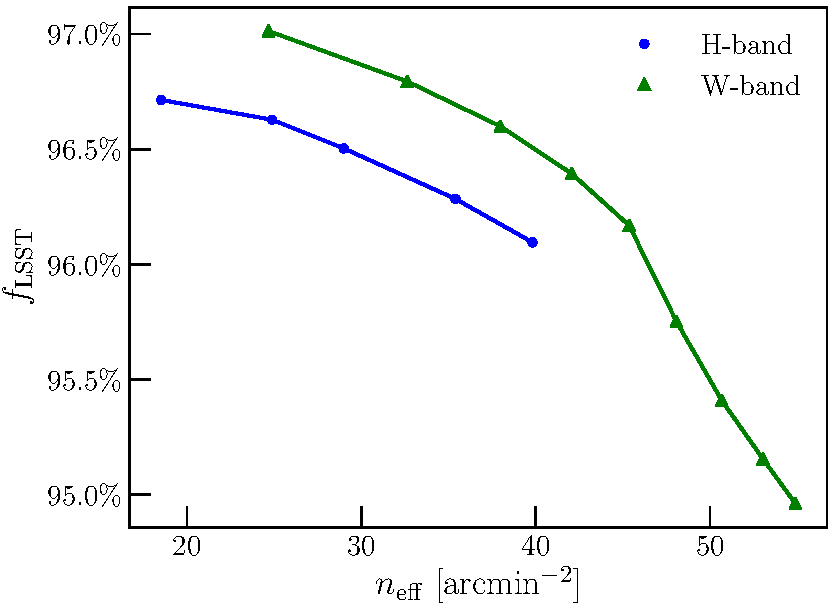
\includegraphics[width=9.5cm]{plots/plot_number_density_with_LSST_redshift.pdf}
 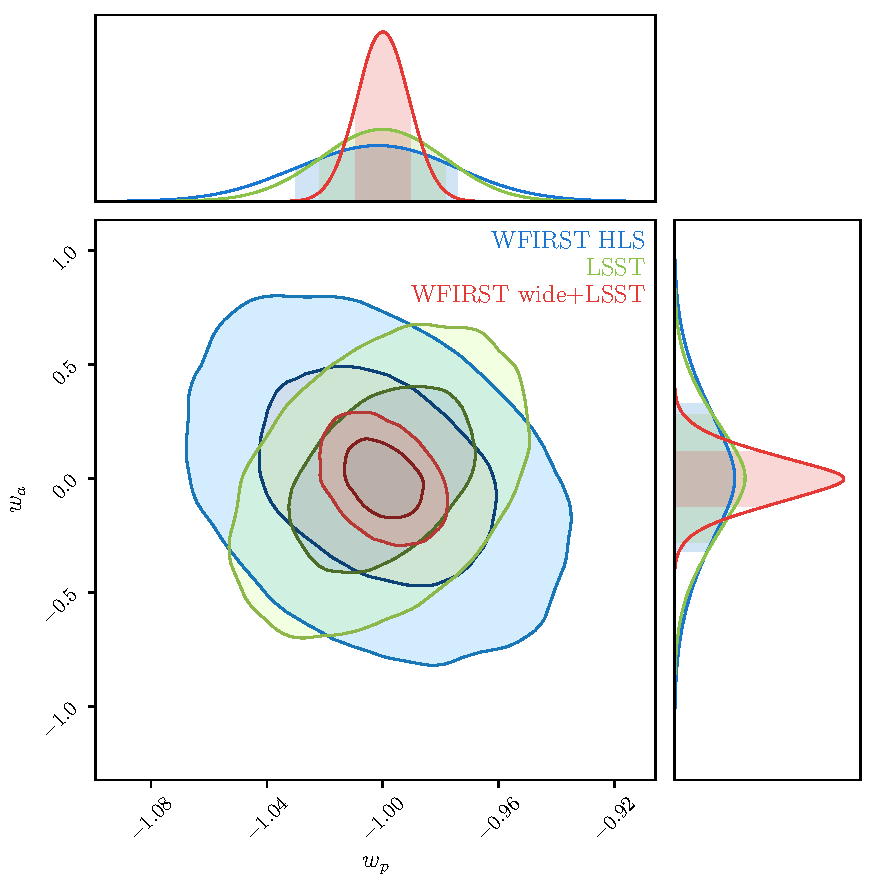
\includegraphics[width=7cm]{plots/WF_LSST_wp06.pdf}
\caption{\textit{Left:} Fraction of LSST galaxies with acceptable multi-band photometry as a function of number density of a WFIRST weak lensing sample, based on the CANDELS catalog. \textit{Right:} Potential gain in constraining power on dark energy parameters $w_p$ and $w_a$, marginalized over 5 other cosmological parameters (no systematics), for a joint data set of LSST multi-band photometry and deep W-band WFIRST imaging over the whole LSST area. }
\label{fi:contour_stats}
\end{figure*}

\todo{Tim - integrate table into text and expand it to reflect the settings on LSST, WFIRST and joint analysis, remove cosmology info}
\renewcommand{\arraystretch}{1.3}
\begin{table}
\caption{Fiducial parameters, flat priors (min, max), and Gaussian priors ($\mu$, $\sigma$)}
\begin{center}
\begin{tabular*}{0.45\textwidth}{@{\extracolsep{\fill}}| c c c |}
\hline
\hline
Parameter & Fid & Prior \\  
\hline 
\multicolumn{3}{|c|}{\tbf{Survey}} \\
$\Omega_{\mathrm{s}}$ & 2,000 deg$^2$ & fixed\\
$n_{\mathrm{eff}}$ & 50 gal/arcmin$^2$ & fixed\\
$\sigma_\epsilon$ &0.26& fixed\\
\hline 
\multicolumn{3}{|c|}{\tbf{Cosmology}} \\
$\om$ & 0.3156 &  flat (0.1, 0.6)  \\ 
$\sig$ & 0.831 &  flat (0.6, 0.95)  \\ 
$\ns$ & 0.9645 & flat (0.85, 1.06)  \\
$\w$ &  -1.0 &   flat (-2.0, 0.0)   \\
$\wa$ &  0.0 &  flat (-2.5, 2.5)   \\
$\omb$ &  0.0492 &  flat (0.04, 0.055)  \\
$h_0$  & 0.6727 &  flat (0.6, 0.76)   \\
\hline
\multicolumn{3}{|c|}{\tbf{Galaxy bias (tomographic bins)}} \\
$b_\mr{g}^i$ & 1.3 + i $\times$ 0.1  & flat (0.8, 3.0) \\
\hline
\multicolumn{3}{|c|}{\tbf{Lens photo-z }} \\
$\Delta_\mr{z,lens}^i $ & 0.0 & Gauss (0.0, 0.0004) \\
$\sigma_\mr{z,lens} $ & 0.01 & Gauss (0.01, 0.0006) \\
\hline
\multicolumn{3}{|c|}{\tbf{Source photo-z}} \\
$\Delta_\mr{z,source}^i $ & 0.0 & Gauss (0.0, 0.002) \\
$\sigma_\mr{z,source}$ &0.05 & Gauss (0.05, 0.003) \\
\hline
\multicolumn{3}{|c|}{\tbf{Shear calibration}} \\
$m_i $ & 0.0 & Gauss (0.0, 0.004)\\
\hline
\end{tabular*}
\end{center}
\label{tab:params}
\end{table}
\renewcommand{\arraystretch}{1.0}

\todo{Tim - update Fig to show the gain with systematics, check that the LSST info reflects the SRD}

The contours in Fig.~\ref{fi:contour_stats} (right) reflect the gain in cosmological constraining power when combining the two surveys compared to each survey alone. We assume conservative scale cuts to shield against astrophysical systematics ($l_{\rm max}=3000$ for LSST lensing, $l_{\rm max}=4000$ for WFIRST lensing, $R_{\rm min}=21$ Mpc/h for galaxy-galaxy lensing and for galaxy clustering in both surveys).

We stress that astrophysical systematics should be included in future studies of such a joint analysis to assess the gain in information, however such studies require a broader consensus in the community of how to parameterize these systematics and which uncertainties (parameter values) to assign. It can be assumed that the improvement in constraining power is even more impressive when including systematics, since a joint analysis of LSST and WFIRST will will enable improved modeling of astrophysics, most importantly galaxy bias, intrinsic alignment, baryonic physics. Future studies should also include probes beyond the 3x2pt analysis presented here.

Figure \ref{fi:contour_stats} (right) shows the substantial increase in statistical precision when combining the LSST data set with a 1.5 year WFIRST wide W-band survey. This improvement stems from a combination of higher number density of galaxies \citep[see][for a detailed study]{2019arXiv190108586S}, deeper redshift distribution of source and especially lens galaxies. It would be interesting to explore the information gain for LSST as a function of WFIRST survey time as an extension of this study.

We again emphasize that this white paper does not recommend replacing the current 2000 deg$^2$ HLS survey with a wide W-band survey of WFIRST. The current design of the HLS ensures exquisite systematics control and it is the consensus in the community that systematics control will be more important than maximizing statistical power. We instead recommend the exploration of the WFIRST wide survey strategies in combination with the HLS approach, specifically we envision that a wide WFIRST survey component would use the reference HLS to anchor shear and photo-z calibration.  


\section{Synergies between WFIRST and LSST beyond 3x2 science}
By the time WFIRST launches, LSST will have been in survey mode for several years already and will have built up substantial survey depth and area. The science collaborations of LSST will know precisely what limits the precision of their core science cases and what type of observations are neccessary/most interesting. WFIRST with its broad range of capabilities will be an ideal partner observatory to LSST at exactly the right time.

For cosmology and dark energy science from LSST it is not unlikely that blending of source galaxies will be a limiting systematic for LSST shape and photo-z measurements. It is also possible that the lack of deep training data (spectra) for photo-z, or the lack of multi-band IR coverage will limit LSST photo-z accuracy. If blending proves to be a limiting issue, the 5-month WFIRST wide survey is an important idea to study further. If the lack of spectroscopic information is limiting, exploring the idea of extended WFIRST grism observations is interesting. If narrow band IR information is useful, a WFIRST wide survey with the H-band is interesting to study. 

In terms of how to fit the wide survey into the WFIRST mission, several options arise: one is an extended mission, which is well-matched in terms of timescale to LSST Y10. A second option is to get the wide survey data earlier and to reduce the 2000 deg$^2$ of HLS in the primary mission. A third option would be to do a subset of the 18,000 deg$^2$ in the WFIRST primary mission, e.g. one could survey 10,400 deg$^2$ with E(B-V)$<$0.08 that pass within 32 degrees of zenith at LSST. This will likely be the best part of the LSST footprint for extragalactic studies, and it can be surveyed in 58$\%$ of the time indicated by the x-axes of Fig. \ref{fi:wbanddepth}. In this context we note that the WFIRST observing time, including the survey design of the HLS, has not been allocated to date, and that corresponding decisions will depend on the science landscape in $\sim$5 years. 

A WFIRST wide survey in one band as described above opens numerous science applications in cosmology beyond the joint weak lensing and galaxy clustering dark energy science depicted in Fig. \ref{fi:contour_stats}: 
\begin{itemize}
\item {\bf  Galaxy cluster science:} An 18,000 deg$^2$ W-band survey would substantially enhance the weak-lensing mass calibration of clusters, a key ingredient for cluster cosmology.  Both the increased spatial resolution and the broader wavelength coverage will help to decrease systematic uncertainties due to blending and photo-z misclassification, which are amplified in overdense cluster fields.  An important aspect is that the W-band addition would enable precise mass calibration to higher redshift clusters than LSST alone.
% \item {\bf CMB cross correlations:} The increased number density of galaxies and precision in shape measurements from space-based imaging over the full LSST area would enable a new level of cross-correlation measurements with contemporary CMB experiments (e.g., Simons Observatory, CMB-S4). This would apply to cross-correlations of galaxy clustering and CMB lensing, and galaxy shapes and CMB lensing. Similarly, tSZ observations from CMB surveys will detect a wealth of clusters, all of which benefit strongly from cluster mass calibration through high-precision weak lensing. 
\item {\bf Trough cosmology:} Cosmic underdensities have emerged as a powerful probe of structure formation and hence dark energy and modified gravity; potentially corresponding observables are easier to model compared to probes that rely on higher-density environments. Trough cosmology, and especially trough lensing, would benefit from the 18,000 deg$^2$ wide WFIRST survey scenario because of the higher density of source galaxies (for trough lensing) and the higher density of detected galaxies that signify the trough boundaries. 
\item {\bf Strong Lensing:} LSST will find an enormous number of strong lenses. Color and more importantly shape information from overlapping space observations will allow for substantially improved constraints on cosmology, simply because of the enhanced control of lens profile modeling uncertainties.
\end{itemize} 

\subsection*{Combining WFIRST, LSST and CMB surveys}

The new generation of cosmic microwave background (CMB) experiments, e.g. the Simons Observatory (SO) and CMB-S4, will be well underway by the mid-2020s. In particular, the survey of the Large Aperture Telescope of 	the Simons Observatory over the full LSST footprint \citep{Ade:2019kq} will likely be completed or near completion, providing a detailed map of small-scale secondary CMB anisotropies through CMB lensing (reaching a signal-to-noise ratio above 1 for all multipoles $\ell<200$), the Sunyaev-Zeldovich' (SZ) effect and the cosmic infrared background. The increased number density of galaxies and precision in shape measurements from space-based imaging from WFIRST over the full LSST area would therefore enable a new level of cross-correlations measurements between galaxy surveys and CMB surveys.

The CMB lensing kernel function,
\begin{equation}
\label{eq:qkappa}
q_{\kappa_{\rm CMB}}(\chi) = \frac{3 H_0^2 \Omega_m }{2 \mathrm{c}^2}\frac{\chi}{a(\chi)}  \frac{\chi^*-\chi}{\chi^*} \,.
\end{equation}
peaks at $z\sim2$ and is sensitive to all large-scale structures between the observer and the last scattering surface (here $\chi^*$ is the comoving distance to this surface).
Measurements of cross-correlations of galaxy clustering and shapes with CMB lensing would strongly benefit from the higher density of galaxies of a joint catalog, which will in turn be beneficial to constraints on cosmic acceleration in several ways.
First, extra cosmological information is held in these cross-correlations, which can alleviate parameters degeneracies, for instance between galaxy clustering biases and cosmological parameters. Second, these measurements will enable further cross-calibration of shear multiplicative biases, as shown in \cite{2017PhRvD..95l3512S}, and other nuisance parameters such as uncertainties on photometric redshifts. Third, the joint catalog will have higher density of galaxies at high redshifts \red{(is this true??? IR band + better shapes and deblending should make it possible, right?)}. Therefore, the high redshift tomographic bins will  correlate even more strongly with CMB lensing. At last, the comparison of constraints obtained from subsets of these high-precision cross-correlation measurements will enable various tests of the consistency of the cosmological model with all observables, or reveal potential tensions.

Similarly, thermal SZ observations from CMB surveys will detect a wealth of clusters (16,000 clusters forecasted for SO), all of which benefit strongly from cluster mass calibration through high-precision weak lensing. The more accurate photometry of the joint catalog would improve the redshift determination of these clusters and extend the redshift range of clusters for which both CMB and optical/infrared observations are matched. This will also enable improved measurements of cluster profiles and features such as the splashback radius observed in density and lensing profiles. 

Finally, the increased number density at high redshift will allow correlations with the cosmic infrared background to study the star formation rate of high redshift galaxies \red{(need to check that, too.)}.


\section{Conclusions}

Many of the WFIRST science cases will build on the existing LSST data set. Especially for cosmology, where the existing LSST data are highly complementary to the planned WFIRST science, this will be the case. It is however important to note that this partnership is mutually beneficial and that exploring optimal joint science strategies for WFIRST and LSST deserves serious consideration, calculations, and meaningful metrics. We recommend the exploration of WFIRST survey strategies as a function of potential results and possible limitations from LSST data (taking into account DESI, PFS, SPHEREx, Euclid) and development of optimal joint systematics mitigation concepts that allow WFIRST and LSST to create the legacy data set that will shape cosmology well into the 2030s. 






\section*{Acknowledgments}


\bibliographystyle{mnras}
\bibliography{references.bib}

\end{document}












